%Only the basic operator norms of table \ref{table:OperatorNorm} for $q \sleq p$ are considered for the calculation of the Block-MCC$_{q,p}$ as the similarity measure between the blocks $\myPhi [k]$, and Block-MCC$_{1,\infty}$ is selected in showing the results.

Assuming that the number of clusters is not known, a strategy will be needed to appropriately estimate it, which leads us to hierarchical clustering analysis.
Hierarchical clustering 
%groups data in different scales, which 
can be visualized by the so-called clustering tree or dendrogram.
The clustering tree is composed of nodes (clusters) and branches, which the length of each branch shows the distance between the two nodes.
%located at its two ends.
%Then, the number of intersections of a horizontal line with the clustering tree gives the number of clusters in that scale or clustering level.
A scale with the largest distance between consecutive nodes or longest branch can be considered as an appropriate scale for clustering, which gives the estimated number of clusters.
The agglomerative hierarchical clustering algorithm is used. 
In 
%bottom-up or 
agglomerative as opposed to 
%top-down or 
divisive method, each single data is considered as a cluster, then at each clustering level the clusters are successively merged until all the data are clustered into a single cluster.

Suppose that in figure \ref{fig:NumberOfClusters_Estimation}(a), each block $\myPhi [k]$ of dictionary is represented by a single circle, and there are 100 blocks, i.e., $k \ssin \{ 1 , \cdots , 100 \}$.
The relative distances between circles are determined by the proposed coherence measure Block-MCC$_{2,2}$.
The random dictionary is generated in a way to have five equally-sized clusters of blocks of length 20.
Then, $\myPhi [1] , \cdots , \myPhi [20]$, construct cluster I and so on.
The process of generating desired random dictionaries is explained in Section \ref{sec:Artificial simulated dictionary}.
%There are different methods to compute the distance between two clusters.
A method called \emph{complete} has been used to compute the distance between two clusters, which is equal to the longest distance between two points in the two clusters as illustrated in figure \ref{fig:NumberOfClusters_Estimation}(a).
In figure \ref{fig:NumberOfClusters_Estimation}(b) the dendrogram resulted from clustering the random dictionary is shown.
As expected, the magenta dotted horizontal line in the scale with the largest distance between consecutive nodes intersects the dendrogram five times, so the estimated number of clusters is five, which is true.
\begin{figure}[!b]
\centering
\includegraphics[width=1\textwidth,keepaspectratio]{images/NumberOfClusters_Estimation.png} % width=0.5\textwidth  scale=0.49
\centering
\caption{(a) The longest distance between two points in the two clusters determines inter-cluster distance; (b) Number of vertical branches at a clustering level with longest branch approximates the number of clusters.}
\label{fig:NumberOfClusters_Estimation}
\end{figure}
\FloatBarrier
%------------------------------------------------------
\subsection{Synthetic dictionary}
\label{sec:Artificial simulated dictionary} 
Dictionaries $\myPhi \ssin \mathbb{R}^{m \stimes n}$, with equally-sized blocks of length $d_1 \seq \cdots \seq d_K \seq d$, are generated from independent and identically distributed (i.i.d.) random variables and all columns of the dictionaries are normalized to have unit $\ell_2$ norm.
The idea to generate the whole dictionary is first to start from an initial block, next some representative blocks of clusters are generated, then from each representative block of a cluster, the blocks belonging to the same cluster are produced.
To construct a second block from a first one, the random matrix $\exp((\boldsymbol{C} \sm \boldsymbol{C}^T) \sqrt{2} \varepsilon / \Vert \boldsymbol{C} \sm \boldsymbol{C}^T \Vert_F)$ is multiplied to the first block, where, $\boldsymbol{C}$ is a square random matrix of dimension $m$.
Depending on the role of $\varepsilon$ whether to generate representative blocks of clusters or blocks of dictionary, it is named $\varepsilon_{inter}$ or $\varepsilon_{intra}$, respectively.

%To generate a random dictionary, first an initial block of dimension $m$ by $d$ is considered.
%Then, to create $N$ representatives of clusters $\boldsymbol{\mu}^1 , \cdots \boldsymbol{\mu}^N$,
In figure \ref{fig:Dictionary_generating}, the process of generating a random dictionary $\myPhi$ with $N$ clusters and $K$ blocks is illustrated.
First, from a random initial block $\boldsymbol{\mu}^0 \ssin \mathbb{R}^{m \stimes d}$, $N$ representatives of clusters $\boldsymbol{\mu}^1 , \cdots , \boldsymbol{\mu}^N$ are created, using the mentioned multiplier and parameter $\varepsilon_{inter}$.
Then, from each representative $\boldsymbol{\mu}^i$, $\forall i$, the blocks $\myPhi^i\mybracket{j}$, $\forall j$, belonging to the same cluster $i$ are generated, using the mentioned multiplier and parameter $\varepsilon_{intra}$.
The parameter $\varepsilon$ in the multiplier controls the amount of overlap and similarity between blocks.
In fact, $\varepsilon_{inter}$ defines the overlap between the representative blocks of clusters, whereas $\varepsilon_{intra}$ controls the overlap between the blocks belonging to the same cluster.
%It is possible to control the amount of overlap and similarity between blocks of the dictionary by tuning the parameters $\varepsilon_{inter}$ and $\varepsilon_{intra}$, which the former parameter defines the overlap between the average block of each cluster whereas the latter controls the overlap between the blocks belonging to the same cluster.  
%Finally, length of blocks before clustering, number of rows and number of columns of the dictionary are equal to $2$, $10$, and $80$, respectively.
Finally, the results are shown in terms of average and standard deviation over 100 repetitions of random dictionary $\myPhi \ssin \mathbb{R}^{10 \stimes 80}$ generation with $d_j \seq 2$, $\forall j$.
\begin{figure}[!b]
\centering
\includegraphics[width=1\textwidth,keepaspectratio]{images/Dictionary_generating.png} % width=0.5\textwidth  scale=0.49
\centering
\caption{From initial block $\boldsymbol{\mu}^0$, $N$ representative blocks of clusters are computed. Then, from each representative block $\boldsymbol{\mu}^i$, all blocks $\myPhi^i\mybracket{j}$ belonging to the same cluster $i$ are generated.}
%Assuming $N$ clusters and $K$ blocks, $\boldsymbol{\mu}^i$ is the representative block of cluster $i$, and $\myPhi^i\mybracket{j}$ is the block $j$ belonging to cluster $i$ resulted from multiplication of a n $\varepsilon$-based matrix 
%, where based on the value of $\varepsilon$, resulted matrices can have certain amount of overlap with the one originated from.}
\label{fig:Dictionary_generating}
\end{figure}
\FloatBarrier
%------------------------------------------------------
\paragraph{Block-ERC in clustered representation and the number of clusters}
%\subsubsection{Effect of clustering the coherent blocks of a dictionary on Block-ERC based on Block-MCC$_{q,p}$}
\label{sec:clusteringOFcoherent_BERC-BMIC} 
%In general the recovery conditions can be improved or weakened through increasing the required number of non-zero entities as a threshold which ensures the uniqueness of the solution to an optimisation problem.
%In Corollary \ref{crl:BERC-BMIC} of Section \ref{sec:BERC_BNSP}, the mentioned threshold or $\myBSLTxt$ is expressed as the number of blocks (not the number of elements) in two cases of optimistic and pessimistic.
%In Section \ref{sec:Sparsity level for clustered blocks of a dictionary}, we explained how different sparsity levels can be calculated from $\myBSLTxt$, 
% of a Block-ERC, which upper-bounds the maximum number of active blocks of representation vector $\mybeta$ ensuring the uniqueness of the solution to an optimisation problem. 
%which upper-bounds the maximum number of active blocks in a Block-ERC.

In this experiment, 
%$\myBSLTxt$ resulted from a Block-ERC based on Block-MCC$_{q,p}$ is going to be investigated in clustered representation.
%To this purpose, 
the agglomerative hierarchical clustering algorithm is applied on the blocks of a random dictionary with certain number of clusters, whereas the Block-MCC$_{2,2}$ and complete method are used to measure the inter-blocks coherence and inter-clusters distance, respectively.
The mentioned certain number of clusters is once set to four and once set to eight.

As it can be seen in figure \ref{fig:SL_Hierarchical}, by applying hierarchical clustering on the blocks of the dictionary, i.e., by decreasing the number of clusters, there exists at least one clustering level in which the relative $\myBSLTxt_{2,2}$ in the most pessimistic case, i.e., $\myBSL_{2,2}(\myPhi)[\%]$, increases in comparison to when the clustering is not applied on the dictionary, i.e., the rightmost part of each diagram corresponding to 40 clusters.
Therefore, clustering coherent blocks of the dictionary improves the Block-ERC through increasing the $\myBSLTxt_{2,2}$.

In addition, for $\varepsilon_{inter} \sg 1$ and $\varepsilon_{intra} \sless 0.1$, the $\myBSL_{2,2}(\myPhi)[\%]$ has a peak in a clustering level equal to the number of the clusters in the simulated dictionary.
In fact, in figure \ref{fig:SL_Hierarchical} when there is four clusters in the simulated dictionary (blue curve, square markers), the maximum is at the fourth clustering level and also the consistent results are obtained for eight clusters in the dictionary (red curve, circle markers).
For the clustering level lower than the optimal level, the space is under-sampled and there would be a block spanning the whole space, whereas for the clustering level higher than the optimal level, the space is over-sampled and the over-partitioning leads to high coherence measure.
\begin{figure}[!b]
\centering
\includegraphics[width=1\textwidth,keepaspectratio]{images/SL_Hierarchical.png} % width=0.5\textwidth  scale=0.49
\centering
\caption{$\myBSL_{2,2}(\myPhi)[\%]$ for each level of clustering computed for complete method, Block-MCC$_{2,2}$, $d \seq 2$, $N \seq \{ 4 , 8\}$, and different values of $\varepsilon_{inter}$ and $\varepsilon_{intra}$ for simulating dictionary $\myPhi \ssin \mathbb{R}^{10 \stimes 80}$.}
\label{fig:SL_Hierarchical}
\end{figure}
\FloatBarrier
%------------------------------------------------------
\paragraph{Block-ERC in clustered representation and the conventional ERC}
%\subsubsection{Sparsity level in a clustered blocks compared to the conventional sparsity level}
In this experiment, the goal is to compare the sparsity level obtained in the proposed Block-ERC to the conventional sparsity level which is equal to the half of the number of rows of $\myPhi$.%the dictionary.

First, we need to express the block-sparsity level in terms of the conventional sparsity level as described in Section \ref{sec:Sparsity level for clustered blocks of a dictionary}, e.g., $\mySLTxt_{min}$ and $\mySLTxt_{max}$.
Then, consider one of the cases in figure \ref{fig:SL_Hierarchical}, e.g., $\varepsilon_{inter} \seq 3.5$, $\varepsilon_{intra} \seq 0.1$.
% and complete method.
So, the complete method is used to calculate inter-clusters distance, whereas the Block-MCC$_{2,2}$ measures the inter-blocks coherence of a dictionary $\myPhi \ssin \mathbb{R}^{10 \stimes 80}$ with equally-sized blocks, i.e., $d_1 \seq \cdots \seq d_{40} \seq d \seq 2$.

In figure \ref{fig:SL_Hierarchical_conventional}, it can be seen that by applying hierarchical clustering on the blocks of the dictionary, the increase in the sparsity levels even surpasses the conventional sparsity level which is marked with a black dotted line.
It can be seen in figure \ref{fig:SL_Hierarchical_conventional} that close to the clustering level equal to the number of clusters in the simulated dictionary, even the proposed $\mySLTxt_{min}$ can surpass the conventional sparsity level.
Therefore, clustering the coherent blocks of a dictionary in addition to enhancing the Block-ERC through increasing the $\myBSLTxt_{2,2}$, improves the conventional sparsity level. 
Hence, improves the conventional ERC.

At last, in order to make sure that the clustering structure in a clustering level, where, there is a peak in sparsity level is done properly, the average clustering accuracy over 100 repetitions is computed for fourth (for the case of four clusters in the dictionary) and eighth (for the case of eight clusters in the dictionary) clustering levels, which are equal to \myhl{$99.65\%$} and \myhl{$100\%$}, respectively.
Therefore, the peak in the sparsity level diagram, which is more striking in figure \ref{fig:SL_Hierarchical} in addition to giving an estimation of the number of clusters in the dictionary, also with \myhl{high probability (at least in this example)} corresponds to the correct clustering structure of the dictionary.
\begin{figure}[!b]
\centering
\includegraphics[width=.95\textwidth,keepaspectratio]{images/SL_Hierarchical_conventional.png} % width=0.5\textwidth  scale=0.49
\centering
\caption{$\mySLTxt_{min}[\%]$ and $\mySLTxt_{max}[\%]$ for each level of clustering computed for complete method, Block-MCC$_{2,2}$, $d \seq 2$, $\varepsilon_{inter} \seq 3.5$ and $\varepsilon_{intra} \seq 0.1$ for (a) $N \seq 4$ and (b) $N \seq 8$ in the dictionary $\myPhi \ssin \mathbb{R}^{10 \stimes 80}$.}
\label{fig:SL_Hierarchical_conventional}
\end{figure}
\FloatBarrier
%------------------------------------------------------
\subsection{Real EEG/MEG lead-field}
\label{sec:Real EEG/MEG leadfield} 
In this experiment the hierarchical clustering is used because of its characteristic in estimation of the number of clusters, as described in section \ref{sec:hierarchical_cluster_estim}.
In order to simulate or import real-world sensor, source and volume conduction head model required to generate the real lead-field we used an open source software package MATLAB-based toolbox named FieldTrip \cite{Oostenveld2011}.

EEG lead-field is obtained using 32 standard electrodes and utilising three different volume conduction head models of three-layer concentric spheres, realistic three-layer with inflated cortical sheet obtained by boundary element
methods and realistic three-layer with highly-folded cortical sheet obtained by SPM8 software \cite{SPM}.
Realistic head models are obtained by imposing anatomical constraint, which is provided by MRI\footnote{\emph{Magnetic Resonance Imaging}}.

Similarly, for MEG lead-field generating, 32 standard sensors closest to the previously selected 32 EEG standard electrodes are selected and single sphere, realistic single layer with inflated and highly-folded cortical sheets are used as volume conduction head models.
The sensor model, three-compartment (brain, skull, and scalp) volume conduction head model (analytical and realistic), and source model (spherical and realistic) are shown in figure \ref{fig:Sensor_vol_Source}. 
\begin{figure}[!b]
\centering
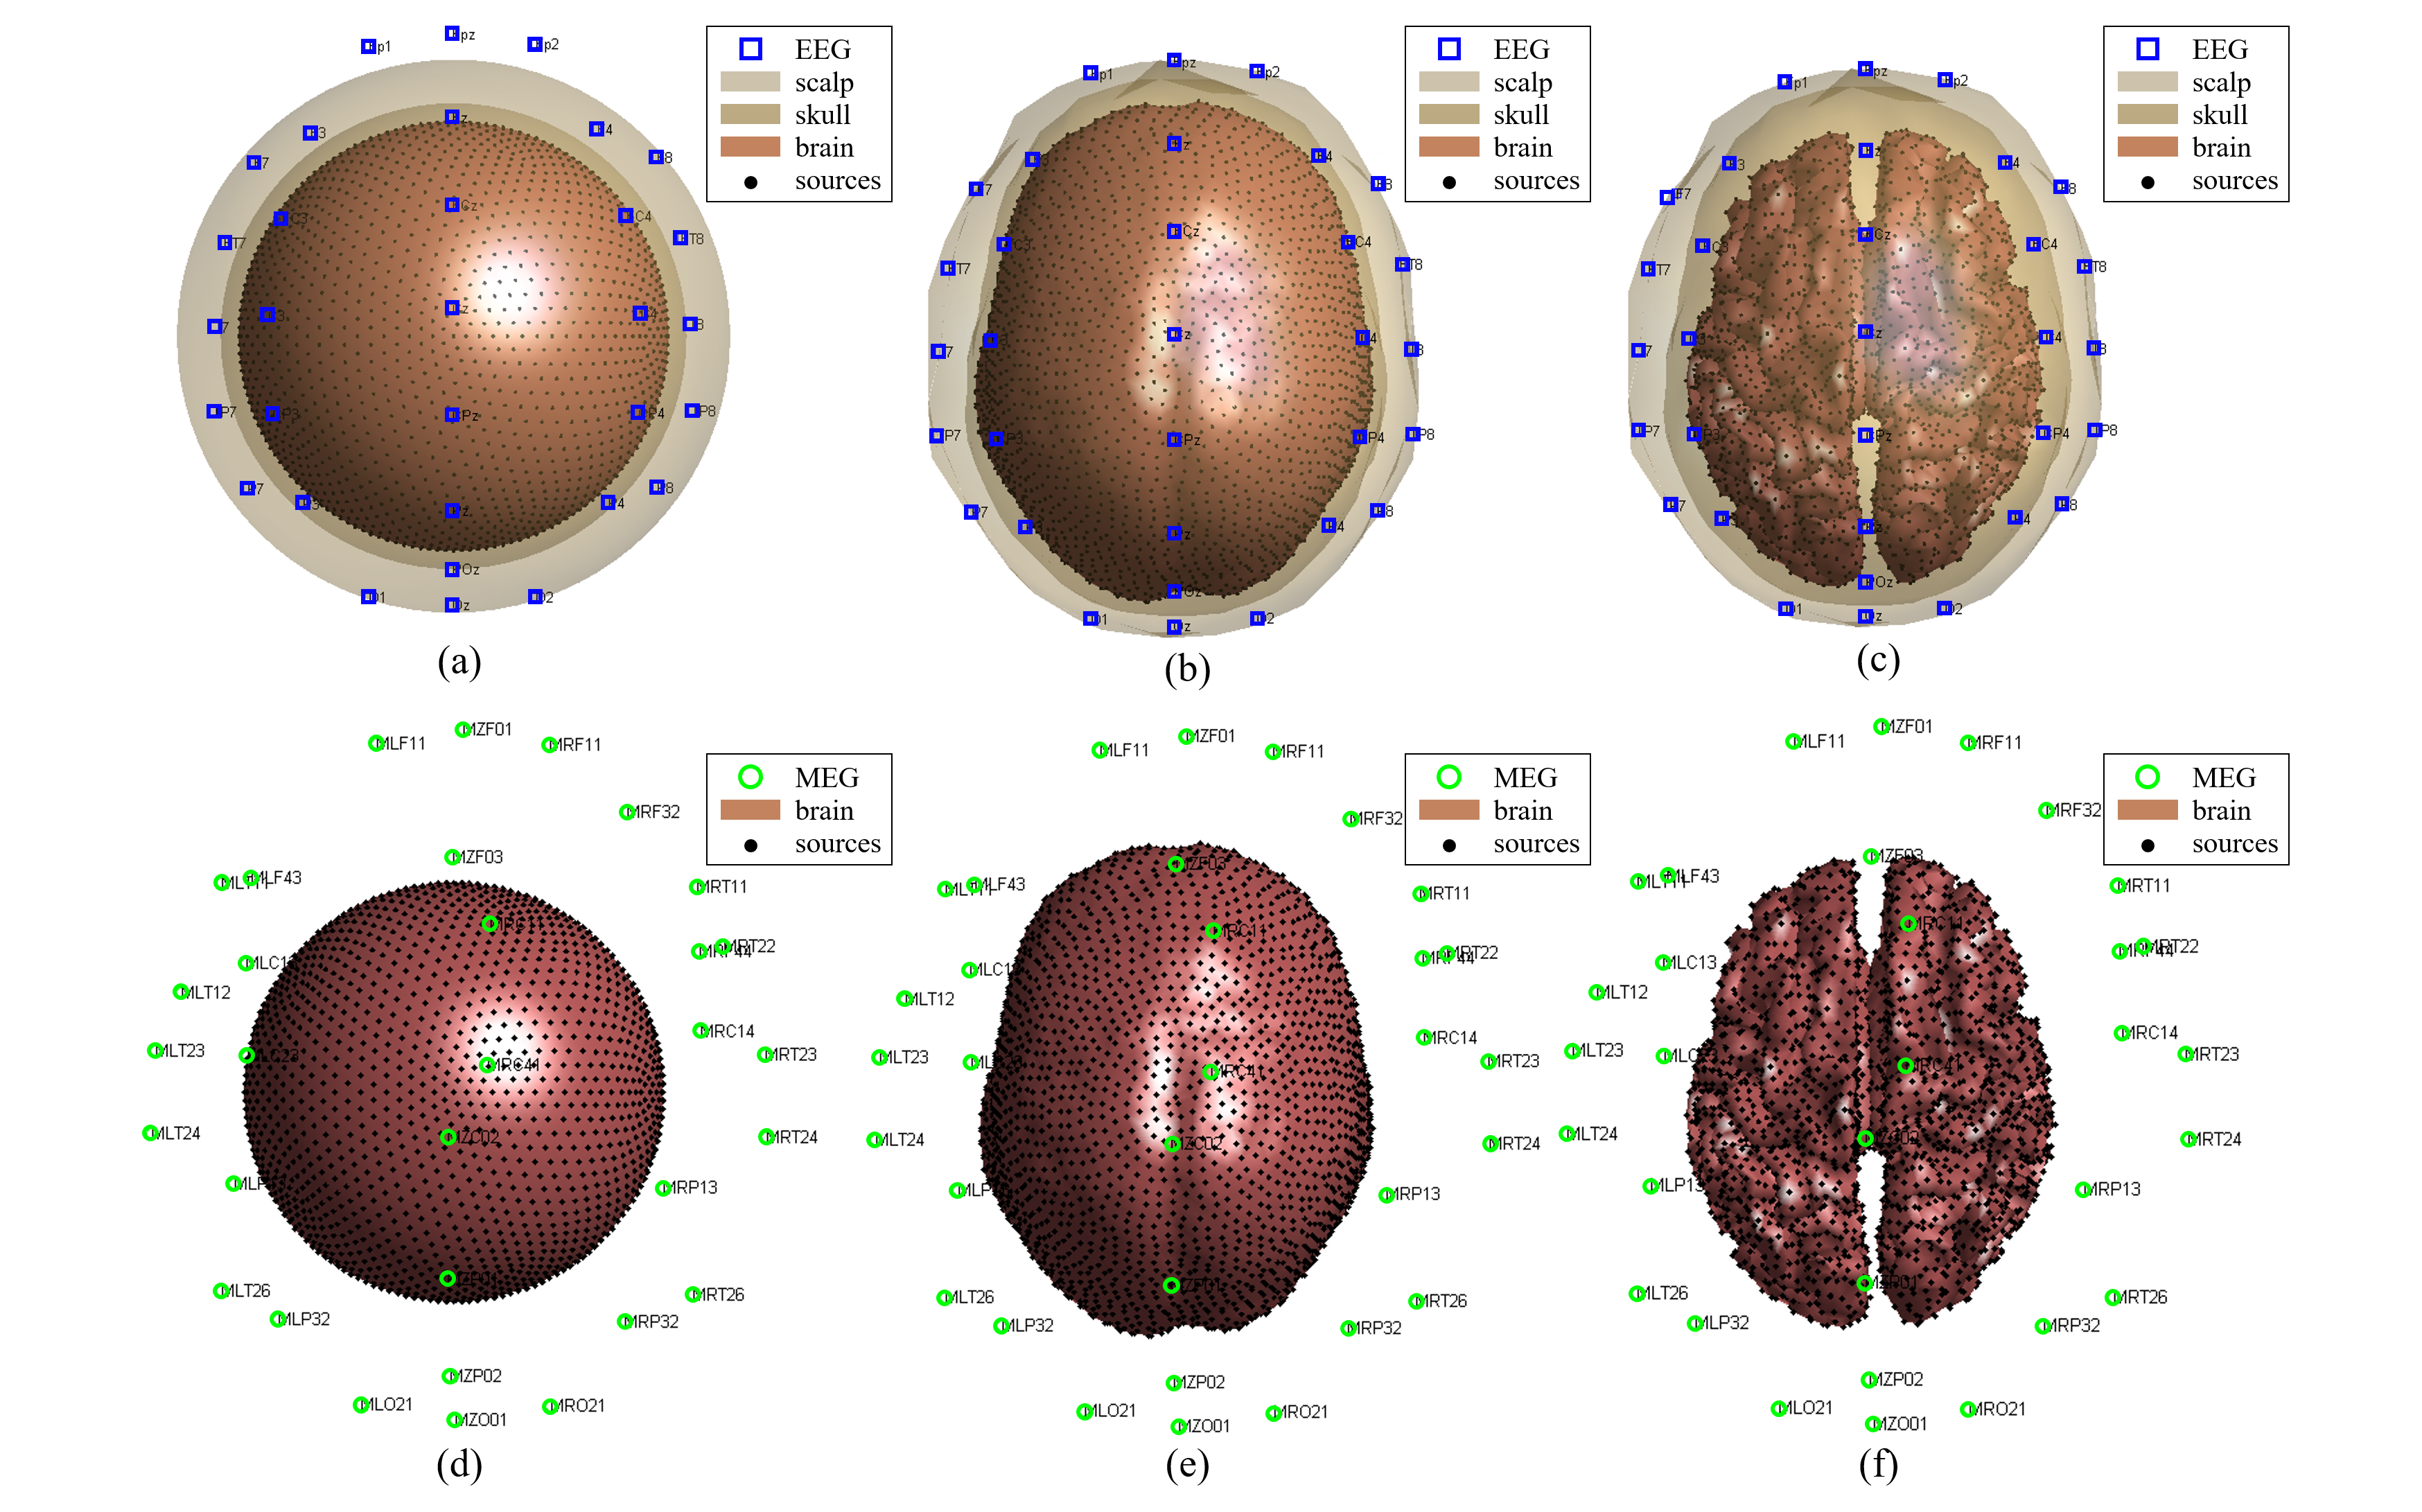
\includegraphics[width=1\textwidth,keepaspectratio]{images/Sensor_vol_Source.png} % width=0.5\textwidth  scale=0.49
\centering
\caption{Different geometrical models of the EEG/MEG experiment: 1- Spherical (a,d), realistic inflated (b,e), and realistic highly-folded (c,f) source models; 2- EEG (a,b,c), and MEG (d,e,f) sensor models; 3- Three-layer concentric spheres (a), realistic three-layer (b,c), single sphere (d), and realistic single layer (e,f) volume conduction head models.}
\label{fig:Sensor_vol_Source}
\end{figure}
\FloatBarrier
%------------------------------------------------------
%\subsubsection{Sparsity level in a clustered blocks compared to the initial unclustered blocks}
\paragraph{Block-ERC in clustered representation}
As explained in Section \ref{sec:Sparsity level for clustered blocks of a dictionary}, generally, in transforming the $\myBSLqpTxt$, which is determined by Block-ERC, into the conventional sparsity level, different types of sparsity levels can be appeared, e.g., minimum sparsity level 
%in the most pessimistic case 
$\mySLTxt_{min}$, and maximum sparsity level 
%in the most pessimistic case 
$\mySLTxt_{max}$.
%, minimum sparsity level in the most optimistic case $\mySLTxt^{opt}_{min}$, and maximum sparsity level in the most optimistic case $\mySLTxt^{opt}_{max}$.
On the other hand, as described earlier in the Section \ref{sec:hierarchical_cluster_estim}, number of branches in a clustering level with maximum inter-node distance in a clustering tree resulted from a hierarchical clustering algorithm can be used as an estimation of the number of clusters of a dictionary.

Assume the sparsity level computed in the clustering level corresponding to the maximum inter-node distance in the clustering tree is shown by $\mySLTxt_2$, whereas the sparsity level computed for the lead-field without clustering is called $\mySLTxt_1$.
In order to investigate the effect of clustering the coherent blocks of the lead-field on sparsity levels, we compute the relative change quantity, i.e., $(\mySL_2(\myPhi) \sm \mySL_1(\myPhi)) {/} \mySL_1(\myPhi)$.

In figure \ref{fig:EMEG-LF-clustering-SL}, the relative change of sparsity levels $\mySLTxt_{min}$, and $\mySLTxt_{max}$ is shown.
%, $\mySLTxt^{opt}_{min}$, and $\mySLTxt^{opt}_{max}$ is shown.
In addition, the experiment is repeated for two modalities of EEG and MEG, and three head models with spherical, realistic inflated and realistic highly-folded cortical sheets.

As it can be seen in figure \ref{fig:EMEG-LF-clustering-SL}, by clustering coherent blocks of the lead-field (whether EEG/MEG or spherical/realistic cortical sheet) using the proposed Block-MCC$_{2,2}$, all sparsity levels significantly increase, especially $\mySLTxt_{max}$.
% and $\mySLTxt^{opt}_{max}$.
Hence, clustering coherent blocks of lead-field using the proposed Block-MCC$_{q,p}$ coherence measure leads to improved Block-ERC.

%In addition to the segmentation effect mentioned in previous part, the relative improvement of $\mySLTxt^{pes}_{min}$, $\mySLTxt^{pes}_{max}$, $\mySLTxt^{opt}_{min}$, and $\mySLTxt^{opt}_{max}$ in the estimated clustering level in comparison to the last level of clustering where the number of clusters is equal to the number of blocks, is shown in figure \ref{fig:EMEG-LF-clustering-SL} as bar charts, which indicates a significant increase on values, i.e., clustering coherent blocks of leadfield results in weakened recovery conditions.
\begin{figure}[!b]
\centering
\includegraphics[width=0.9\textwidth,keepaspectratio]{images/EMEG-LF-clustering-SL.png} % width=0.5\textwidth  scale=0.49
\centering
\caption{Relative increase of sparsity levels $\mySLTxt_{min}$, $\mySLTxt_{max}$, 
%$\mySLTxt^{opt}_{min}$, and $\mySLTxt^{opt}_{max}$, 
when clustering the coherent blocks of lead-field, repeated for two modalities of EEG and MEG, and three head models with spherical, realistic inflated and realistic highly-folded cortical sheets.}
\label{fig:EMEG-LF-clustering-SL}
\end{figure}
\FloatBarrier
%------------------------------------------------------
\paragraph{EEG/MEG source space segmentation}
As described in Section \ref{sec:EMEG segmentation}, clustering the coherent blocks of the lead-field matrix results in some brain regions, because each block of the lead-field correspond to \myhl{a single source position in the source space.}
Then, coherent source positions form brain regions, where, coherency is defined by the Block-MCC$_{q,p}$ coherence measure applied on the bocks of the lead-field.

The results of clustering coherent source positions using EEG and MEG lead-field, and for three head models with spherical, realistic inflated and realistic highly-folded cortical sheets are shown in figure \ref{fig:EMEG-LF-clustering-regions}. 
Although, in this experiment the number of clusters or brain regions is estimated from the clustering tree, but since there is a series of clustering structures in the hierarchical clustering analysis, by introducing extra information to the problem about the number of brain regions, there would be the possibility of having different brain regions.
In other words, the resulted brain regions in figure \ref{fig:EMEG-LF-clustering-regions} are not fixed and can be adapted based on the number of regions.
In addition, the resulted brain regions are a function of Block-MCC$_{q,p}$ and inter-cluster distance method.


%By clustering the blocks of the leadfield matrix, coherent sources form clusters, hence brain regions appear as described in Section \ref{sec:EMEG segmentation} and the number of clusters can be estimated by counting the number of intersections of a horizontal line with the dendrogram in an area where there is the maximum distance between adjacent nodes.

%Using Block-MCC$_{1,\infty}$ as the similarity measure and the complete method as the algorithm for computing the distance between clusters, the brain source space segmentation resulted from EEG leadfield clustering in three cases of one spherical and two realistic volume conduction head models can be seen in figure \ref{fig:EMEG-LF-clustering_regions}(a), (b), and (c), respectively.
%As it can be seen in figure \ref{EMEG-LF-clustering-regions}(a), with the help of dendrogram it is possible to estimate the number of clusters and the clustering structure.
%Similar results are obtained from MEG leadfield, which are shown in figure \ref{EMEG-LF-clustering-regions}(d), (e) and (f).
\begin{figure}[!b]
\centering
\includegraphics[width=1\textwidth,keepaspectratio]{images/EMEG-LF-clustering-regions.png} % width=0.5\textwidth  scale=0.49
\centering
\caption{Brain source space segmentation, when clustering the coherent blocks of lead-field, repeated for two modalities of EEG and MEG, and three head models with spherical, realistic inflated and realistic highly-folded cortical sheets.}
\label{fig:EMEG-LF-clustering-regions}
\end{figure}
\FloatBarrier
%------------------------------------------------------
\paragraph{Comparison to the conventional lobes of the brain}
In order to compare the resulted brain source space segmentation in a specific clustering level to the conventional lobes of the brain, the closest boundaries to the conventional boundaries are shown in figure \ref{fig:Atlas}(a) and (b).

The brain segmentation and boundaries resulted from EEG, and MEG lead-fields are shown in figure \ref{fig:Atlas}(a), and (b), respectively.
The anatomical lobes and the functional areas of the brain are shown in figure \ref{fig:Atlas}(c).

Therefore, using the proposed framework, i.e., clustering coherent blocks of the lead-field with the help of the proposed Block-MCC$_{q,p}$ coherence measure, the conventional structural and functional brain lobes can be divided into subject-specific refined regions.
\begin{figure}[!b]
\centering
\includegraphics[width=1\textwidth,keepaspectratio]{images/Atlas.png} % width=0.5\textwidth  scale=0.49
\centering
\caption{The proposed subject-specific brain source space segmentation, using (a) EEG, and (b) MEG lead-fields, compared to (c) the conventional anatomical and functional brain lobes.}
\label{fig:Atlas}
\end{figure}
\FloatBarrier